\section{Técnica de evaluación de fiabilidad}\label{sec:tecnicas_evaluacion_fiabilidad}
La evaluación de la fiabilidad es de suma importancia para el desarrollo de sistemas críticos, ya
que permite identificar que aspectos del comportamiento del sistema juega un papel importante
\citep{FTDesign}.

\begin{enumerate}
 \item Modelado de un sistema en la fase de diseño.
 \item Aseguramiento del sistema en la fases finales de desarrollo (testing).
\end{enumerate}
El análisis confiabilidad tiene tres enfoques importantes:
\begin{itemize}
  \item Confiabilidad de \ac{HW}
  \item Confiabilidad de \ac{SW}
  \item Confiabilidad humana
\end{itemize}
En este trabajo de tesis se pondrá énfasis en el estudio en la confiabilidad del \ac{SW} a nivel de sistema.

La evaluación de la fiabilidad tiene dos aspectos. En primer lugar se tiene una \textit{evaluación
cualitativa} que permite identificar, clasificar y medir modos de fallas, o eventos combinacionales
que puedan provocar una falla. El otro aspecto es la \textit{evaluación cuantitativa}, la cual
permite evaluar en términos de probabilidad los atributos de la fiabilidad, disponibilidad, seguridad (Sección \ref{sec:atributos_de_la_fiabilidad}).

El análisis de confiabilidad es de gran importancia ya que provee información que es la base de la toma de desiciones.
Esto es aplicado a diferentes áreas, tales como análisis de riesgos, protección ambiental, calidad, optimización de mantenimientos y operaciones y diseño de ingeniería \citep{Rausand04}.

\section{Medidas comunes de fiabilidad}\label{sec:medidas_fiabilidad}
Las medidas de fiabilidad más comunes son las siguientes: failure rate, tiempo medio a la falla,
tiempo medio de reparación y tiempo medio entre fallas.

\subsection{Failure rate}
Failure rate $\lambda$ es el número esperado de fallas por unidad de tiempo \citep{FTDesign}. Es
usual utilizar la dimensión \textit{fallas/horas}.

Generalmente, $\lambda$ se encuentra a nivel de componente. Para conocer el failure rate del
sistema completo, se puede realizar (\textit{grosso modo}) una sumatoria de los $\lambda$ de los
componentes que integran el sistema. $$\lambda=\sum_{i=1}^{n} \lambda_i$$.

La evolución de $\lambda$ a través del tiempo, no tiene el mismo comportamiento tanto para \ac{HW} como para \ac{SW}.
Si se divide el ciclo de vida de un sistema en las siguientes fases: mortalidad prematura (I), vida útil (II), desgaste (II) \citep{FTDesign}
se aprecia, para el caso del \ac{HW}, lo que se denomina \textit{curva de la bañera} la cual puede observarse en la Figura \ref{fig:bathtub_curve}.
En una primera fase, $\lambda$ decrese, ya que a través de los procesos de testing se van descubriendo y resolviendo los errores. Luego se da un periodo de estabilización.
Y al final, el \ac{HW} sufre el paso del tiempo, y se desgasta, aumentando la tasa de fallas.

\begin{figure}[h]
 \centering
 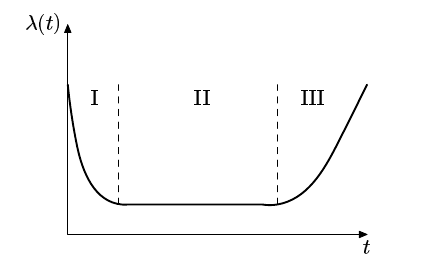
\includegraphics[scale=0.5]{images/Marco_teorico/bathtub_curve.png}
  \caption{Failure rate de HW vs tiempo }
\label{fig:bathtub_curve}
\end{figure}

Para el \ac{SW} es totalmente diferente. En primer lugar cuando se realiza una actualización, se aumenta la complejidad, como así también la probabilidad de fallas,
con ello el failure rate. Otra diferencia sustancial con el \ac{HW} es que el \ac{SW} no se desgasta con el tiempo. En la Figura \ref{fig:Failure_rate_software}
se puede apreciar $\lambda$ a través de tiempo. Esta curva suele llamarse \texit{curva serrucho}. El failure rate del \ac{SW} decrece en función del tiempo. En estos tipo de sistemas
la tasa de falla depende de varios factores como pueden ser el proceso utilizado en el diseño y codificación, complejidad del \ac{SW}, tamaño del \ac{SW},etc \citep{FTDesign}.

\begin{figure}[h]
 \centering
 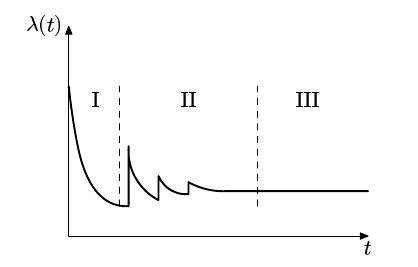
\includegraphics[scale=0.5]{images/Marco_teorico/Failure_rate_software.png}
  \caption{Failure rate SW vs tiempo }
\label{fig:Failure_rate_software}
\end{figure}

A lo largo de la vida del sistema se supon que el failure rate $\lambda$ es constante. Por lo tanto la confiabilidad del sistema varía exponencialmente
con respecto al tiempo \citep{FTDesign}: $$R(t) = e^{- \lambda t}$$

Esto se conoce como \textit{ley de la falla exponencial} \citep{FTDesign}. El gráfico de confiabilidad $R(t)$ vs tiempo se muestra en la Figura \ref{fig:failure_rate}.

\begin{figure}[h]
 \centering
 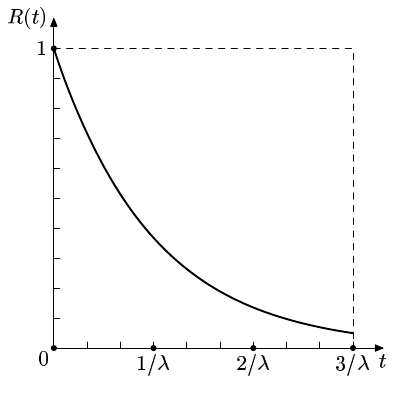
\includegraphics[scale=0.5]{images/Marco_teorico/failure_rate.png}
  \caption{Confiabilidad vs tiempo }
\label{fig:failure_rate}
\end{figure}

\subsection{Tiempo medio de falla}
\textit{El tiempo medio de falla} (MTTF\footnote{Del inglés, Mean Time To Failure}) de un sistema es el tiempo esperado que transcurra hasta la primera falla que se
detecte en el sistema. En terminos de confiabilidad, MTTF se define de la siguiente manera (\citep{FTDesign}; \citep{Rausand04}) $$\int_0^{\infty} R(t) dt$$

\subsection{Tiempo medio de reparación}
\textit{El tiempo medio de reparación} (MTTR\footnote{Del inglés, Mean Time To Repair})
de un sistema, es el promedio de tiempo que se requiere para reparar al sistema.
MTTR se especifica en términos de la tasa de reparación $\mu$ (\citep{FTDesign}; \citep{Rausand04}), el cual es el número esperarado de reparaciones por unidad de tiempo: $$MTTR = \frac{1}{\mu}$$

El MTTR depende de los mecanismos de recuperación ante fallas que se utilicen en el sistema, localización del sistema, scheduler de mantenimiento \citep{FTDesign}. Con esto se puede definir la disponibilidad como sigue: $$A(\infty) = \frac{MTTF}{MTTF+MTTR}$$

Muchas veces se utiliza MDT\footnote{Del inglés, Meann Downtime} en vez de MTTR, para denotar más claro que es el tiempo medio que el sistema se encuentra fuera de servicio.

\subsection{Tiempo medio entre fallas}
\textit{El tiempo medio entre fallas} (MTBF\footnote{Del inglés, Mean Time Between Failure}) de un sistema es el tiempo promedio entre dos fallas del sistema. $$MTBF = MTTF + MTTR$$

\subsection{Cobertura de fallas}
La cobertura de fallas es la probabilidad  de que el sistema no interrumpirá su actividad cuando una falla se presente. En términos matemáticos la cobertura
de fallas es la probabilidad condicional $P(A|B)$. Existen diferentes coberturas de fallas, dependiendo de si se está tratando con detección de fallas, localización de fallas, contención de
fallas o recuperación de fallas \citep{FTDesign}. Siendo $A$ detección, localización, contensión o recuperación de fallas, y $B$ la existencia de fallas.

\section{Métodos de cálculos de fiabilidad}\label{sec:metodos_calculo_confiabilidad}
Para evaluar la fiabilidad de sistemas se pueden utilizar diagramas de bloque de confiabilidad y procesos de Markov \citep{FTDesign}

\subsection{Diagramas de bloques de confiabilidad}

\subsubsection{Cálculo de confiabilidad}
Para medir la confiabilidad de un sistema mediante diagrama de bloques, se debe dividir el sistema objetivo en  partes paralelas y en serie. Se computa la confiabilidad
de las partes. La confiabilidad del sistema estará compuesta por la confiabilidad de ambas partes \citep{FTDesign}. Entonces
$$R(t) = \left \{
\begin{matrix}
  \prod_{i=1}^{n} R_{i}(t) & \text{para estructuras en serie}\\
  1 - \prod_{i=1}^{n}(1-R_{i}(t)) & \text{para estructuras en paralelo}
\end{matrix} $$
Esto nos indica que un sistema paralelo, es más confiable que uno en serie, aún así si sus componentes son menos confiables. Tal como ejemplifica \cite{FTDesign}, si se diseña un sistema en serie de 100 componentes, con una confiabilidad de 0.999, el sistema completo tendrá una confiabilidad de:
$0.999^{100} = 0.905$. Mientras que, para un sistema paralelo, con solo cuatro componentes, con una confiabilidad menor (0.95) la confiabilidad del sistema
será $1-(0.95)^4 = 0.99999375$. El punto en contra de los sistemas paralelos, es que representan un costo mayor que las estrucuturas en serie \citep{FTDesign}.

\subsubsection{Cálculo de disponibilidad}
Si se asume que el tiempo de falla y de recuperación son independientes, entonces se puede utilizar diagramas de bloques para calcular la disponibilidad
del sistema  \citep{FTDesign}.  Se puede observar que el cálculo es similiar al calculo de confiabilidad.
 $$A(t) = \left \{
 \begin{matrix}
   \prod_{i=1}^{n} A_{i}(t) & \text{para estructuras en serie}\\
   1 - \prod_{i=1}^{n}(1-A_{i}(t)) & \text{para estructuras en paralelo}
 \end{matrix} $$

\subsection{Utilización de procesos de Markov}
El principal objetivo del análisis de los procesos de Markov es calcular $P_i(t)$ la probabilidad de que el sistema se encuentre en el estado $i$
en el tiempo $t$. Con esto se puede calcular facilmente la confiabilidad, disponibilidad o seguridad del sistema \citep{FTDesign}.

Para determinar $P_i(t)$ se debe derivar una serie de ecuaciones diferenciales, una por cada estado del sistema. Estas ecuaciones se denominan ecuaciones de estado de transición. Las ecuaciones de los estados de transición se representan en una matriz $M$ denominada \textit{matriz de transición}. Cada elemento $m_{ij}$ de la matriz $M$ es un rate de transición entre los estados $i$ y $j$
$$M = \left [
\begin{matrix}
  m_{11}  & m_{12}  & ... & m_{k1} \\
  m_{12}  & m_{22}  & ... & m_{k2} \\
          &         & ... &        \\
  m_{1k}  & m_{2k}  & ... & m_{kk} \\
\end{matrix}
\right ]
$$

Haciendo $P(t)$ un vector en el cual el $i-ésimo$ elemento es la probabilidad $P_i(t)$ de que el sistema se encuentra en el estado $i$ en el tiempo $t$. Con ello se tiene: $$\frac{d}{dt}P(t) = MP(t)$$ \citep{FTDesign}.

Para calcular confiabilidad, disponibilidad y seguridad solo es necesario reemplazar en la matriz $M$, los rate correspondientes.
